\documentclass[article]{IEEEtran}
\usepackage[brazilian]{babel}
\usepackage[utf8]{inputenc}
\usepackage{cite}
\usepackage{geometry}
\usepackage{graphicx}
\usepackage{amsmath}
\graphicspath{{./images/}}
\usepackage{float}
\usepackage[hyphens,spaces]{url}

\begin{document}

%
% paper title
% Titles are generally capitalized except for words such as a, an, and, as,
% at, but, by, for, in, nor, of, on, or, the, to and up, which are usually
% not capitalized unless they are the first or last word of the title.
% Linebreaks \\ can be used within to get better formatting as desired.
% Do not put math or special symbols in the title.
\title{Utilização de fibras ópticas em sistemas de telecomunicação}



% author names and affiliations
% transmag papers use the long conference author name format.

\author{
	Felipe C. S. Santos,
	\and
	Thiago K. Lago
	
\IEEEauthorblockA{Universidade Federal do Rio de janeiro \\ 
	Escola Polit\'{e}cnica \\
	Departamento de Engenharia Eletrônica}
}



\IEEEtitleabstractindextext{
\begin{abstract}

\end{abstract}
\begin{IEEEkeywords}
Telecomunicações, fibras ópticas, optoeletrônica
\end{IEEEkeywords}}



% make the title area
\maketitle

\IEEEdisplaynontitleabstractindextext
As fibras ópticas tem diversas finalidades, sendo uma das mais importantes a utilização em telecomunicações. O avanço das tecnologias de fabricação, modulação e também instrumentação tem tornado cada vez mais viável a utilização das mesmas para transmissões de dados a grandes distâncias com altas taxas de bits. Busca-se através deste paper mostrar o processo de escolha e dimensionamento de uma rede baseada em componentes óticos.
\IEEEpeerreviewmaketitle



\section{Introducão}
\subsection{Elementos do sistema}
\par Qualquer sistema de comunicação pode ser representado pelo diagrama na figura \ref{fig:diagrama-sistema-comunicacao}, este é composto por distintos elementos que possuem as seguintes funções: \cite{FUND_OPT}

\begin{enumerate}
\item \textbf{Fonte:} Responsável pela geração da informação a ser transmitida
\item \textbf{Emissor}: Possui o papel de acoplar a mensagem a um meio de transmissão
\item \textbf{Canal:} É o meio de transmissão em si. Atenua o sinal enviado e insere um ruído. Para comunicação, pode ser o ar, fios ou a fibra óptica.
\item \textbf{Receptor:} Possui a finalidade de tratar a mensagem vinda pelo canal e enviá-la ao destinatário
\item \textbf{Destinatário:} É o destino da mensagem.
\end{enumerate}

\begin{figure}[h]
\label{fig:diagrama-sistema-comunicacao}
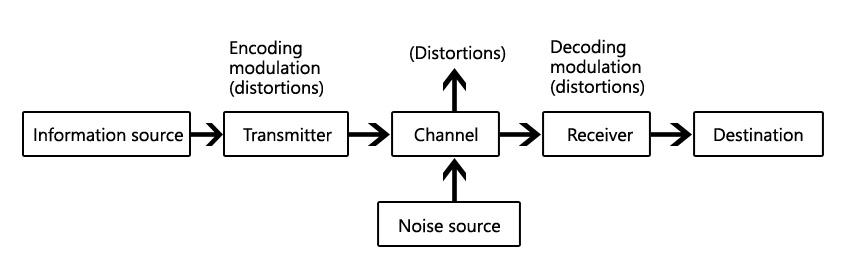
\includegraphics[width=\columnwidth]{communication-system.jpg}
\caption{Diagrama de blocos de um sistema de comunicação}
\end{figure}

Para o caso da fibra óptica, o emissor é uma fonte luminosa, que envia à fibra óptica (o canal) luz. A luz é interpretada no receptor, que pode ser um sensor fotovoltaico. A mensagem agora em pulsos elétricos é enviada ao destinatário e pode ser utilizada como qualquer outra mensagem vinda de um diferente meio de comunicação.
\section{Construção da fibra}


\subsection{Tipos de fibras}

\subsubsection{Fibra monomodo}
Neste tipo de fibra, como o nome sugere, apenas um modo - comprimento de onda - passa pela fibra. Geralmente, o comprimento de onda é referente a segunda ou terceira janela (1310 nm ou 1550 nm). As fibras monomodo possuem uma banda maior e menor perda em relação às multimodo. A restrição de apenas um modo é realizada pois a fibra possui um pequeno core na mesma ordem de grandeza que o comprimento de onda da luz incidente. A desvantagem deste tipo de fibra é que apenas emissores com laser podem fazer acoplamento nesta fibra.

\subsubsection{Fibra multimodo}
Ao contrário da fibra monomodo, a fibra multimodo permitem a passagem de diversos modos. Os comprimentos de onda que são utilizados nessa fibra estão na faixa de 850-1300nm. Neste tipo de fibra, o core possui um diâmetro maior, o que permite a passagem de mais modos. Esta fibra é mais barata em relação à monomodo. E ao projetar o sistema é necessário levar em conta o problema de dispersão modal. Como alguns modos são transmitidos com várias reflexões e outros com poucas, estes modos vão se distanciando. Este efeito distorce o sinal e pode causar problemas na interpretação da mensagem.

\begin{figure}[h]
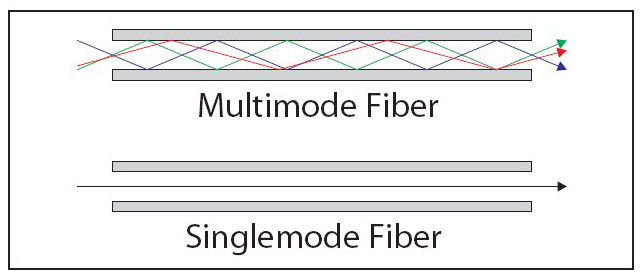
\includegraphics[width=\columnwidth]{mono-multi.jpg}
\caption{Representação das fibras multi e monomodo}
\end{figure}


\subsection{Janelas de transmissão}

\subsubsection{História}
Como é possível ver na figura \ref{fig:hist-window}, entre os anos de 1970 e 1990 houve um grande desenvolvimento no material que compõe as fibras ópticas. Com este avanço surgiram novas janelas de transmissão e isso proporcionou uma menor perda do sinal para longas distâncias.
\begin{figure}[h]
\label{fig:hist-window}
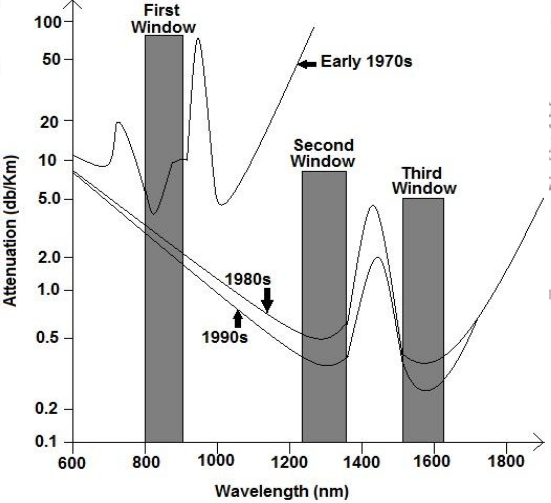
\includegraphics[width=\columnwidth]{hist-windows.png}
\caption{Desenvolvimento das janelas de transmissão em fibras ópticas}
\end{figure}


\subsubsection{Primeira Janela}
Os primeiros sistemas de comunicação com fibra óptica em 1970 utilizavam lasers com comprimento de onda no entorno de 800 nm.
A faixa de transmissão entre 800-900 nm, possui uma perda de sinal de 4dB/km. E como os primeiros sistemas utilizavam esta janela, a mesma ficou conhecida como primeira Janela.
\subsubsection{Segunda Janela}
Com o avanço da tecnologia de purificação do vidro, a segunda  e terceira janelas apareceram. A segunda janela de transmissão é conhecida como banda O, e nela há uma perda de 0.5dB/km e é centrada em 1300 nm. Esta janela possui um suporte a altas taxas de transmissão de dados.
\subsubsection{Terceira Janela}
Atualmente, a maioria dos sistemas de comunicação são feitos utilizando a terceira janela, centrada em 1550 nm e chamada de banda C. Ela possui uma perda de 0.2dB/km, o que é ideal para sistemas de longa distância, pois permite a instalação de amplificadores ópticos mais espaçados.
\section{Componentes ópticos}
Atualmente exitem diversos componentes ópticos que são utilizados durante o projeto de um sistema de comunicação. Os componentes fundamentais para tal sistemas serão citados a seguir.

\begin{figure}[h]
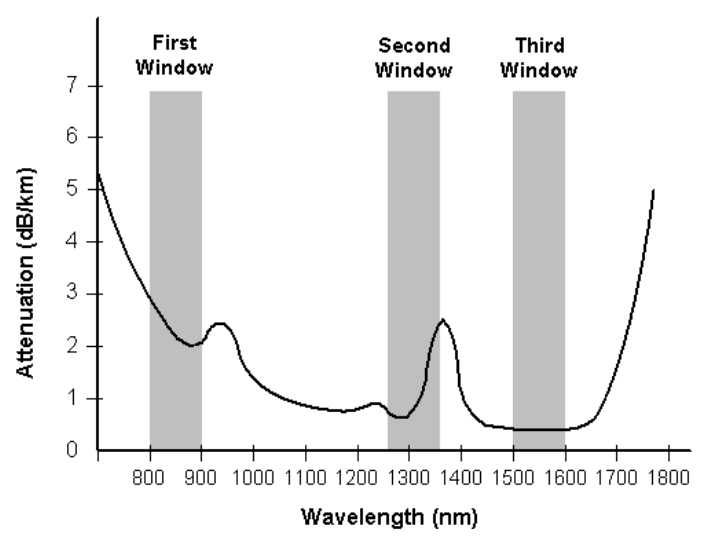
\includegraphics[width=\columnwidth]{windows.png}
\caption{Janelas de transmissão e comprimentos de onda na transmissão}
\end{figure}


\subsection{Transmissores ópticos}
Os principais tipos de transmissores são:
\subsubsection{LED}
Possuem como principal vantagem seu preço, disponibilidade e confiabilidade. A luz é gerada por emissão espontânea, portanto apenas emitem luz incoerente e com amplo espectro. Este tipo de emissor também não é direcional, portanto apenas pode ser acoplado à fibra multimodo e com baixa eficiência.\cite{TRANSMITTERS}
\subsubsection{Diodos de Laser}
Este tipo de diodo possui uma faixa de preço muito mais elevada que o LED. Também são muito sensíveis à temperatura e precisam estar em um ambiente estável para funcionar de maneira ótima. 
Porém este tipo de transmissor possui uma saída mais direcionada que o LED, aumentando assim sua eficiência no acoplamento de fibras ópticas. Este fato também proporciona o uso de fibras ópticas monomodo, aumentando assim a distância alcançada pelo sistema de comunicação. Os diodos lasers, ao contrario do LED, emitem luz coerente portanto a luz é emitida com apenas uma frequência, diminuindo assim a dispersão modal. \cite{TRANSMITTERS}

\subsection{Receptores ópticos}
O receptor óptico é o elemento responsável por detectar a potência óptica incidente e extrair o sinal dela. É um componente crítico pois geralmente determina a eficiência do sistema, e deve manter boas taxas de razão sinal ruido.\cite{RECEIVER}

\subsection{Amplificadores ópticos}
\par Esta tecnologia permitiu um enorme avanço na utilização de fibras ópticas para comunicação em longas distâncias. Antes dos amplificadores ópticos, eram utilizados repetidores eletrônicos. Estes recuperavam o sinal óptico e transformavam a mensagem em sinal elétrico. Este sinal era então amplificado, filtrado, convertido para sinal óptico e finalmente transmitido para a fibra, agora já amplificado. Apesar de possuírem uma boa eficiência, estes repetidores aumentavam o custo do sistema como um todo. Porque possuem uma eletrônica muito complexa, principalmente para transmissões moduladas em altas taxas.
\par Com o avanço da tecnologia de fabricação das fibras, foi possível a criação de amplificadores ópticos, com eles o processo de amplificação é totalmente realizado no domínio óptico. Tornando desnecessário a utilização de amplificadores regenerativos.
\subsubsection{Amplificadores ópticos semicondutores}
Os amplificadores ópticos semicondutores (SOA) amplificam a luz incidente através de emissão estimulada.


\begin{figure}[h]
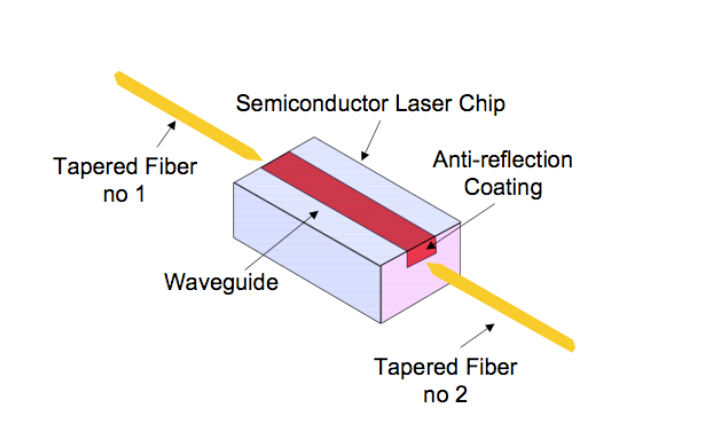
\includegraphics[width=\columnwidth]{soa.jpg}
\end{figure}

A amplificação é obtida bombeando externamente os níveis de energia do material. Para obter apenas a função de amplificação, é necessário proteger o dispositivo contra oscilações próprias, gerando o efeito laser.
Os fótons que passam pela região ativa são estimulados e possuem o mesmo comprimento de onda que o sinal óptico, amplificando assim o sinal óptico durante a passagem pelo dispositivo.


\subsection{Rede de Bragg}
A rede de Bragg, ou em inglês \textit{Fiber Bragg Grating - FBG} possui um elevado número de aplicações. Para os sistemas de comunicação, são utilizadas para filtrar determinados comprimento de onda.

\begin{figure}[h]
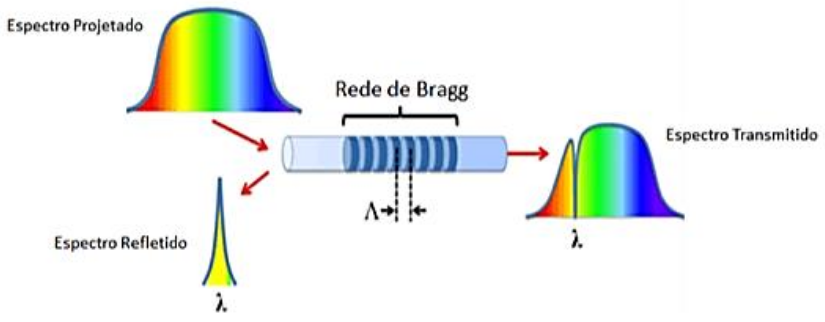
\includegraphics[width=\columnwidth]{fbg-principle.png}
\caption{Funcionamento da Rede de Bragg}
\end{figure}

Utilizando uma FBG em conjunto com um circulador, é possível retirar comprimentos de onda específicos de um sistema de comunicação. A FBG reflete o comprimento de onda desejado e o circulador separa o sinal refletido para uma outra fibra. Esse tipo de sistema pode ser utilizado para separar de uma fibra multimodo informações que sejam específicas para um local sem interferir os outros modos.
\begin{figure}[h]

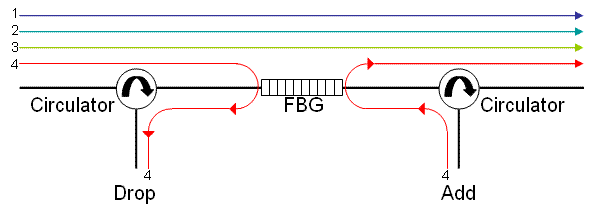
\includegraphics[width=\columnwidth]{Fbg.png}
\caption{Uso da rede de bragg para filtrar modos}
\end{figure}


\section{Modulações utilizadas}
\subsection{Amplitude Shift Keying (ASK)}
\par A modulação ASK (Amplitude Shift Keying) é um tipo de modulação por intensidade do sinal da portadora, também conhecida por ON-OFF-keying. O sinal é modulado em uma portadora óptica de alta frequência. Na técnica ASK, um sinal de frequência da portadora é adicionado ao sinal da mensagem. Logo uma mensagem com o bit 1, é transmitido um sinal com A W. Enquanto que no bit 0 com 0 W. A modulação ASK é simples de gerar e detectar. No ponto de detecção, a demodulação pode ser realizada facilmente utilizando um detector fotovoltaico, que converte a energia óptica em elétrica, resultando o sinal transmitido.
\par	Para um sistema mais avançado de comunicação, é possível atingir mais de um bit transmitido por símbolo. Isto aumenta a capacidade de transmissão e é conhecido como sinalização multinível. De acordo com a equação $M = 2^N$, M representa o nível do sinal e N o número de bits por segundo e é chamado de M-ary signaling.\cite{MODULATION}
\begin{figure}[hb]
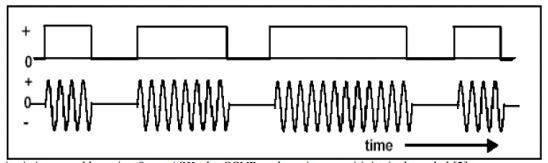
\includegraphics[width=\columnwidth]{ask.png}
\caption{Exemplo de sinal modulado com ASK}
\end{figure}

\subsection{Frequency Shift Keying (FSK)}
\par A modulação FSK é quando a frequência do laser é trocada entre as duas frequências. Nesta técnica de modulação. Comparando com a modulação ASK, a complexidade de gerar e receber do sistema aumenta. Um formato de modulação diferente baseado no FSK pode ser definido mudando valor do índice de modulação. Uma pequena mudança no índice de modulação resulta em um espectro óptico mais compacto. Em sistemas já implantados, um formato de modulação não pode ser substituído pelo formato de modulação baseado em FSK devido à complexidade do sistema receptor. Nesta técnica, os parâmetros do transmissor e os  parâmetros do receptor devem ser idênticos.\cite{MODULATION}

\begin{figure}[hb]
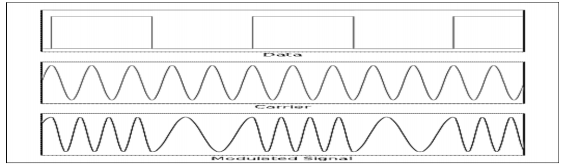
\includegraphics[width=\columnwidth]{fsk.png}
\caption{Exemplo de sinal modulado com FSK}
\end{figure}

\subsection{Phase Shift Keying (PSK)}
\par Phase Shift Keying é a técnica de modulação digital em que a fase da portadora muda, alterando a entrada por senos ou cossenos. Essa modulação possui  dois tipos, a BPSK e QPSK.
\subsubsection{BPSK}
\par Nesta técnica, a portadora senoidal toma duas formas de phase, 0º e 180º.
\subsubsection{QPSK}
\par Nesta técnica, a portadora senoidal pode tomar diversos valores de fase como 0º, 90º, 180º e 270º.

\begin{figure}[h]
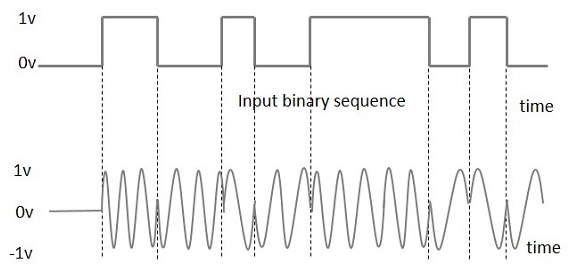
\includegraphics[width=\columnwidth]{psk.png}
\caption{Exemplo de sinal modulado com PSK}
\end{figure}

\subsection{Polarization Shift Keying (PolSK)}
Na modulação PolSK existem dois estados ortogonais de polarização entre o qual o sinal polarizado é mudado para gerar o sinal PolSK. Nesta modulação, o conteúdo do sinal é constante , o que melhora a tolerância não linear e sensibilidade para uma melhor utilização da largura de banda do sistema, a modulação PolSK possui um complexo sistema de geração e detecção de sinais, e também é muito sensível a distúrbios de polarização que podem ocorrer na linha de transmissão.\cite{MODULATION}
\begin{figure}[h]
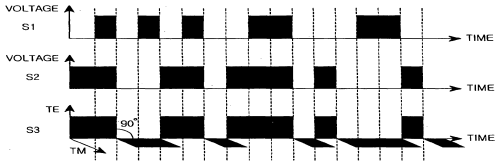
\includegraphics[width=\columnwidth]{polsk.png}
\caption{Exemplo de sinal modulado com PolSK}
\end{figure}

\section{Instrumentros de Medida}
É necessário se preocupar também com a qualidade do sinal recebido e a integridade da fibra óptica. Para isto são utilizados alguns equipamentos que permitem fazer a inspeção das mesmas e analisar o sinal recebido.

Ao instalar uma fibra de grande comprimento, a mesma pode sofrer avarias durante o percurso, prejudicando a recepção do sinal. Outro fator que pode ser determinante na qualidade do sinal recebido é a presença de emendas entre os pedaços das fibras. Existem alguns instrumentos utilizados para resolver este problema. Um deles é o OTDR (\textit{Optical Time Domain Reflectometer}).


\subsection{OTDR}
O \textbf{\textit{OTDR}} utiliza o efeito de retroespalhamento (\textbf{\textit{backscattering}}) dos raios de luz durante a passagem dos sinais luminosos pela fibra óptica. Assim sendo, torna-se possível medir a atenuação do sinal conforme a distância, assim como visto \cite{FOA}

Esse instrumento possui um laser que emite luz em uma frequência pré-determinada e através da diferença de tempo e da potência do sinal medido após o retroespalhamento é possível determinar a relação entre o sinal recebido e a reflexão em uma dada distância de fibra, assim como visto na figura \ref{fig:otdr_esquematico}. Com isso torna-se possível fazer uma inspeção na fibra sem a necessidade de retirar-la do local onde está instalada.

\begin{figure}[H]
	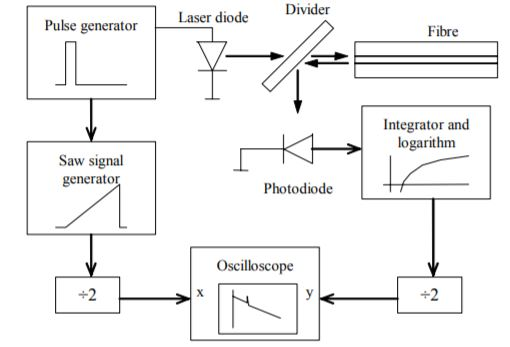
\includegraphics[width=0.5\textwidth]{images/OTDR_esquematico.JPG}
	\caption{Experimento de bancada com OTDR}
	\label{fig:otdr_esquematico}
\end{figure}

O equipamento deve ser conectado conforme a figura [\ref{fig:otdr_teste}], sendo que o cabo de teste pode ter comprimento de alguns quilômetros e ainda sim  pode ser possível realizar a análise com certa clareza. Após uma certa distância, que depende da potência do sinal emitido, da atenuação e reflexão sofrida durante o percurso, o sinal fica num nível comparável ao ruído, conforme visto à esquerda da figura \ref{fig:otdr_teste}:
\begin{figure}[H]
	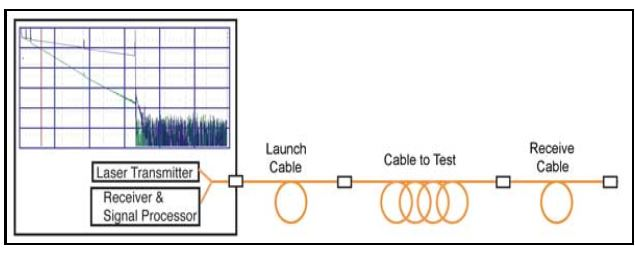
\includegraphics[width=0.5\textwidth]{images/OTDR_teste.JPG}
	\caption{Experimento de bancada com OTDR}
	\label{fig:otdr_teste}
\end{figure}

Uma maneira de aumentar a distância que o sinal chega sem ser muito atrapalhado por ruído é aumentando o comprimento de onda do laser utilizado na inspeção da fibra. Todavia, isto faz com que a resolução do caminho percorrido diminua, sendo assim, obtêm-se menos informação sobre o caminho percorrido pelo sinal. Cabe ao operador do OTDR ajustar o equipamento de forma a obter o melhor compromisso entre distância e resolução, assim como visto em \cite{OTDR_LAB}.

A inclinação da curva na parte linear indica o coeficiente de atenuação da fibra (db/km). Quanto menor a inclinação, mais longe consegue-se transmitir um sinal até que ele chegue à uma razão sinal ruído (\textbf{SNR}) mínima pré-determinada.

Ao utilizar o equipamento para medir a atenuação do sinal conforme a distância da fibra, pode-se observar um gráfico similar ao visto na figura \ref{fig:OTDR_grafico}:
\begin{figure}[H]
	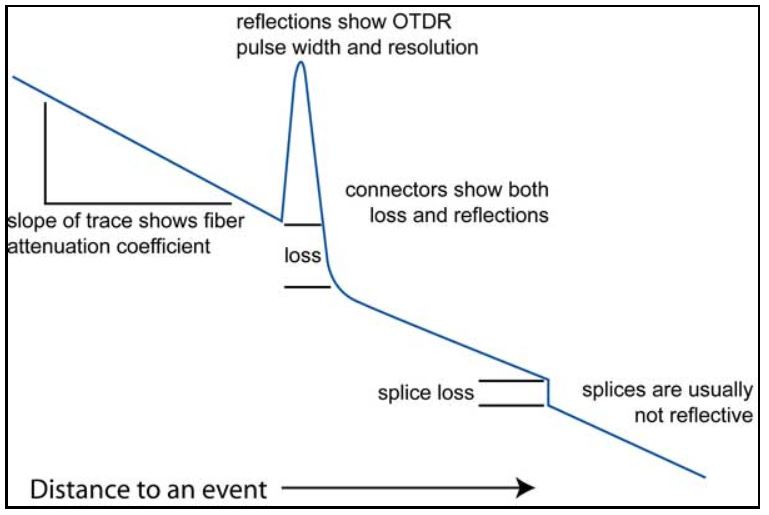
\includegraphics[width=0.5\textwidth]{images/OTDR_grafico.JPG}
	\caption{Experimento de bancada com OTDR}
	\label{fig:OTDR_grafico}
\end{figure} 

Busca-se observar os pontos onde existem descontinuidades na reta de potência do sinal por distância. Estes pontos podem indicar a utilização de um conector mecânico, solda ou até mesmo um rompimento na fibra. Quando a conexão entre fibras é bem feita, a observa-se pouca atenuação no sinal, sendo que a solda bem feita atenua menos que um conector mecânico. Caso observe-se que a inclinação cai bruscamente e o nível do sinal fica próximo ao ruído, pode-se suspeitar de uma fibra rompida ou de uma conexão mal feita.

Existem OTDRs com diferentes finalidades. Antes de fazer a compra do mesmo, necessita-se avaliar o resultado que deseja-se obter com o equipamento. Algumas das perguntas que podem ser feitas são: Há necessidade de ser portátil? Precisa ter bateria? Se precisar, esta deseja-se que esta dure por longo período? A tela precisa ser grande? Qual distância máxima da fibra que desejá-se trabalhar? Qual resolução que se espera nos resultados obtidos? Conforme a pesquisa de preço feito no site mercado livre no dia 30/11/2018 \cite{M_LIVRE}, um OTDR novo pode variar entre R\$3.981, e R\$35.000.

\section{Espectrômetro óptico}
No processo de instalação e configuração de um sistema de telecomunicações baseado em fibras ópticas pode ser necessário analisar a composição espectral da fonte luminosa, dado que o espalhamento das frequências presente no sinal pode significar sobreposição, causando assim erros ao interpretar a informação. Busca-se, na maioria das vezes, utilizar o máximo da fibra em questão de taxa de transmissão, portanto o a frequência que busca-se trabalhar é perto do limiar onde ocorre esta sobreposição.
 
O espectrômetro óptico é um instrumento que tem como finalidade decompor a luz em um espectro de frequência e mostrar este resultado de forma com que se possa realizar análises. Um exemplo de construção é visto na figura \ref{fig:espectrometro_esquematico}

\begin{figure}[H]
	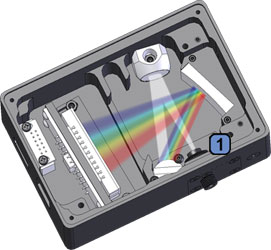
\includegraphics[width=0.5\textwidth]{images/esquematico_espectrometro.jpeg}
	\caption{Esquemático da construção de um espectrômetro óptico}
	\label{fig:espectrometro_esquematico}
\end{figure} 

O caminho que a luz percorre começa pela fenda. Esta pode ser ter diferentes diâmetros. O diâmetro ideal depende do sistema utilizado. Busca-se um balanço entre a quantidade de luz que passa pela fenda e a resolução obtida, assim como visto em \cite{SPECTROMETES}. Após a luz entrar no equipamento,um caminho similar ao mostrado na figura \ref{fig:caminho_luz} é percorrido, passando por um espelho, depois um rede de difração, um outro espelho e chega finalmente a um detector responsável por transformar o sinal luminoso em um valor de intensidade.

\begin{figure}[H]
	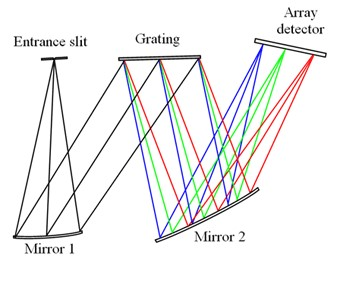
\includegraphics[width=0.5\textwidth, height=0.35\textwidth]{images/caminho_luz.jpg}
	\caption{Caminho da luz dentro do espectrômetro}
	\label{fig:caminho_luz}
\end{figure}  

A rede de difração é um dos fatores determinantes na resolução do espectrômetro. Existem basicamente 2 tipos de redes de difração, sendo que uma delas é mais simples e barata, tendo ranhuras paralelas em sua construção e traz no resultado muita luz difusa. Em algumas aplicações necessita-se que a distribuição espectral seja a mais uniforme possível. Neste caso, a rede de difração holográfica é vantajosa, pois tem uma resposta melhor neste quesito quando comparado com o modelo anterior. A desvantagem desse último modelo é que traz uma eficiência geral bem menor que o primeiro.

Após o processo de reflexão e difração, a luz incide sobre o detector. O CCD é um dos detectores utilizados na construção de um espectrômetro óptico. Os feixes luminosos incidem sobre cada um dos pixels do componente e são transformados em valores de intensidade. Existem materiais com bandas diferentes que podem ser utilizados na construção do detector, assim como visto na figura \ref{fig:materiais_detector}. O tipo ideal para aplicação depende do espectro do sinal que se pretende analisar, assim como também o orçamento do projeto, dado que existem materiais que são mais fáceis de construir, e, portanto, implicam em produtos mais baratos.

\begin{figure}[H]
	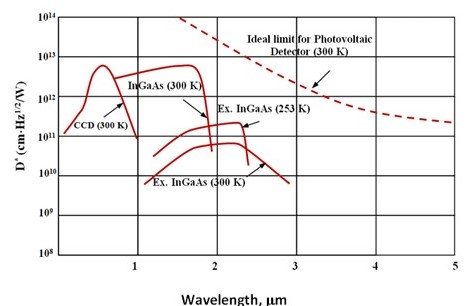
\includegraphics[width=0.5\textwidth]{images/banda_ccd.jpg}
	\caption{Detentividade por comprimento de onda para diferentes materiais}
	\label{fig:materiais_detector}
\end{figure} 

Alguns cuidados devem ser tomado a fim de se obter a medida mais precisa possível. A temperatura deve ser controlada para diminuir o ruído na medida. Isto é feito geralmente através de um cooler termoelétrico construído junto ao equipamento. Outro cuidado é o de garantir que a maior parte da luz incide sobre o detector, pois o se o mesmo tiver pixels com largura menor do que o core da fibra que transmite os sinais, uma parte da luz incidente será perdida. Para isso colocam-se lentes cilíndricas na frente do detector, com a finalidade de focar a luz sem distorcer a imagem formada.

Finalmente, o resultado obtido pode ser parecido com o da figura \ref{fig:resultado_espectrometro}

\begin{figure}[H]
	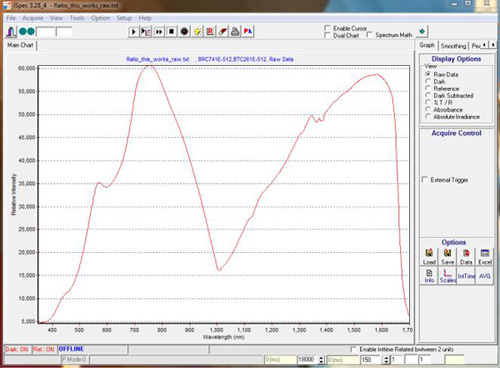
\includegraphics[width=0.5\textwidth]{images/resultado_espectrometro.jpg}
	\caption{Espectro das lâmpadas de tungstênio}
	\label{fig:resultado_espectrometro}
\end{figure} 

\section{Conclusão}
Devido aos avanços tecnológicos na fabricação das fibras ópticas e os componentes que são envolvidos em um sistema de comunicação. A difusão da fibra óptica aumentou consideravelmente. Atualmente, as fibras ópticas garantem a menor atenuação do sinal e podem ser utilizadas para diversas aplicações.
\clearpage
\appendix
\section{Apêndice A}
\subsection{Luz coerente}
\label{ap:l-coerente}
A luz coerente é formada por ondas de mesma frequência e direção, que mantêm uma relação de fase constante. Mais especificamente, dois pontos de uma onda são ditos coerentes quando guardam uma relação de fase constante, ou seja, quando conhecido o valor instantâneo do campo elétrico em um dos pontos, é possível prever o do outro. Existem duas manifestações claramente diferenciadas de coerência: a coerência temporal e a espacial.

\subsubsection{Coerencia temporal}
A coerência temporal está relacionada com a correlação da fase da onda em um determinado ponto alcançado pela mesma em dois instantes de tempo diferentes. Se consideramos o campo elétrico em um ponto P em dois instantes distintos t e t+T se define o tempo de coerência como o máximo valor de T para que a diferença de fase entre o campo em ambos pontos permanece predizível.
\par O elevado índice de coerência temporal dos geradores laser é explorado em diversas aplicações como medidas de distâncias, velocidades, vibrações, etc.
\subsubsection{Coerencia espacial}
A coerência espacial faz referência a uma relação de fase definida entre pontos distintos de uma seção transversal de um feixe luminoso.
A forma de detetar a coerência espacial em um feixe luminoso é mediante o experimento de Young. 
\bibliographystyle{ieeetr}
\bibliography{citations}


\end{document}



